	%% The following is a directive for TeXShop to indicate the main file
%%!TEX root = diss.tex

\chapter{Introduction}
\label{ch:Introduction}

\begin{epigraph}
    \emph{If I have seen farther it is by standing on the shoulders of
    Giants.} ---~Sir Isaac Newton (1655)
\end{epigraph}

Computational Fluid Dynamics (CFD) is a field of study where scientists and engineers architect new ways to numerically solve fluid flow equations. Before the advent of computers, numerical solutions of differential equations was done by hand. This lead to a great deal of work in the direction of creating faster algorithms to solve differential equations. An example is the development of the Fast Fourier Transform (FFT) by Cornelius Lancoz to increase the computation speed of Discrete Fourier Transforms (DFT). However, since the development and advancement of computers, engineers have had a significant amount of compute power to work with. This led to the development of highly accurate methods (as compared to before) to simulate flow over various objects. These simulations have since gotten bigger and better, typically including millions of Degrees Of Freedom (DOF), and now even starting to touch a billion in regular industry use.

\section{Mesh Generation - A Brief Overview}

The equations which govern the conservation of mass, momentum and energy of a moving fluid, called the Navier-Stokes equations, are solved in the given domain to simulate fluid flow in that domain. In order to numerically solve these equations, we need a discretization of the domain. This discrete basis required to solve the Navier-Stokes equations is called a mesh. Simply put, a mesh is a collection of points, lines and cells that together construct the space around a body in a fluid flow. Save a few exotic methods, almost all of the techniques in CFD require a mesh to solve the flow on.

The process of discretization of the domain to form the mesh is called mesh generation. Traditionally, mesh generation was a very manual process, where engineers used to place the mesh points and cells by hand. *todo: add citation and say that this was long time ago.* Such heuristic approach to mesh generation gave them a lot of freedom in discretizing the domain. Cells could be aligned to the boundaries of objects. The quality of the cells, which was taken as some measure of the interior angle of the cells, was almost always chosen to be good. The benefits of this method were quite evident. However, there were some major drawbacks. The process of mesh generation was incredibly slow. Engineers would spend hours, sometime days to create the mesh for a given geometry. Also, mesh adaptation with solution was almost non-existant because that would have made the process even slower.

\begin{definition}
A \textbf{mesh} $M$ is a geometrical discretization of a domain $\Omega$ that consists of (a) a collection of mesh entities $M_i$ of controlled size and distribution and (b) topological relationships or adjacencies forming the graph of the mesh. The mesh $M$ covers $\Omega$ with neither overlaps nor holes.
\end{definition}

\begin{figure}
  \centering
  \begin{subfigure}{0.5\linewidth}
    \centering
    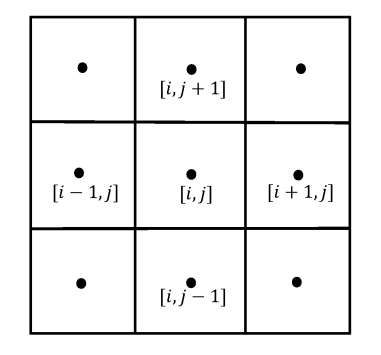
\includegraphics[width=0.8\linewidth]{img/intro/mStructured.png}
    \caption{}
    \label{fig-structured-ij}
  \end{subfigure}%
  \begin{subfigure}{0.5\linewidth}
    \centering
    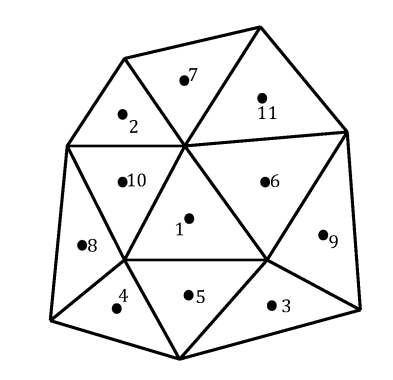
\includegraphics[width=0.8\linewidth]{img/intro/mUnstructured.png}
    \caption{fig-unstructured-ij}
    \label{fig-unstructured}
  \end{subfigure}%
  \caption{}
  \label{fig-structured-unstructured}
\end{figure}

\section{Structured and Unstructured Meshes}

The evolution of mesh generation can be correlated to the evolution of compute power available to the boffins. With the advent of third generation computers (1964-1971) carrying integrated circuits, engineers were able to automate some of the manual processes in mesh generation. Meshes consisting of a template that repeats itself could be generated. These meshes were called \textit{structured meshes} as their adjacencies or relationships could be known implicitly. Consider a grid in two dimensions as shown in Figure \ref{fig-structured-ij}. Given a cell $(i,j)$ we can identify its neighbours as $(i-1, j)$ to the left and $(i+1, j)$ to the right. Similarly, cell $(i, j+1)$ will be to the top and $(i, j-1)$ would be to its bottom. The connectivity pattern repeats in such a mesh. Figure \ref{fig-structuredNaca0012} shows a structured mesh generated for NACA 0012 airfoil around its leading edge. Notice the implicit connectivity of the cells even though the size of mesh elements is varying.

\begin{figure}
  \centering
  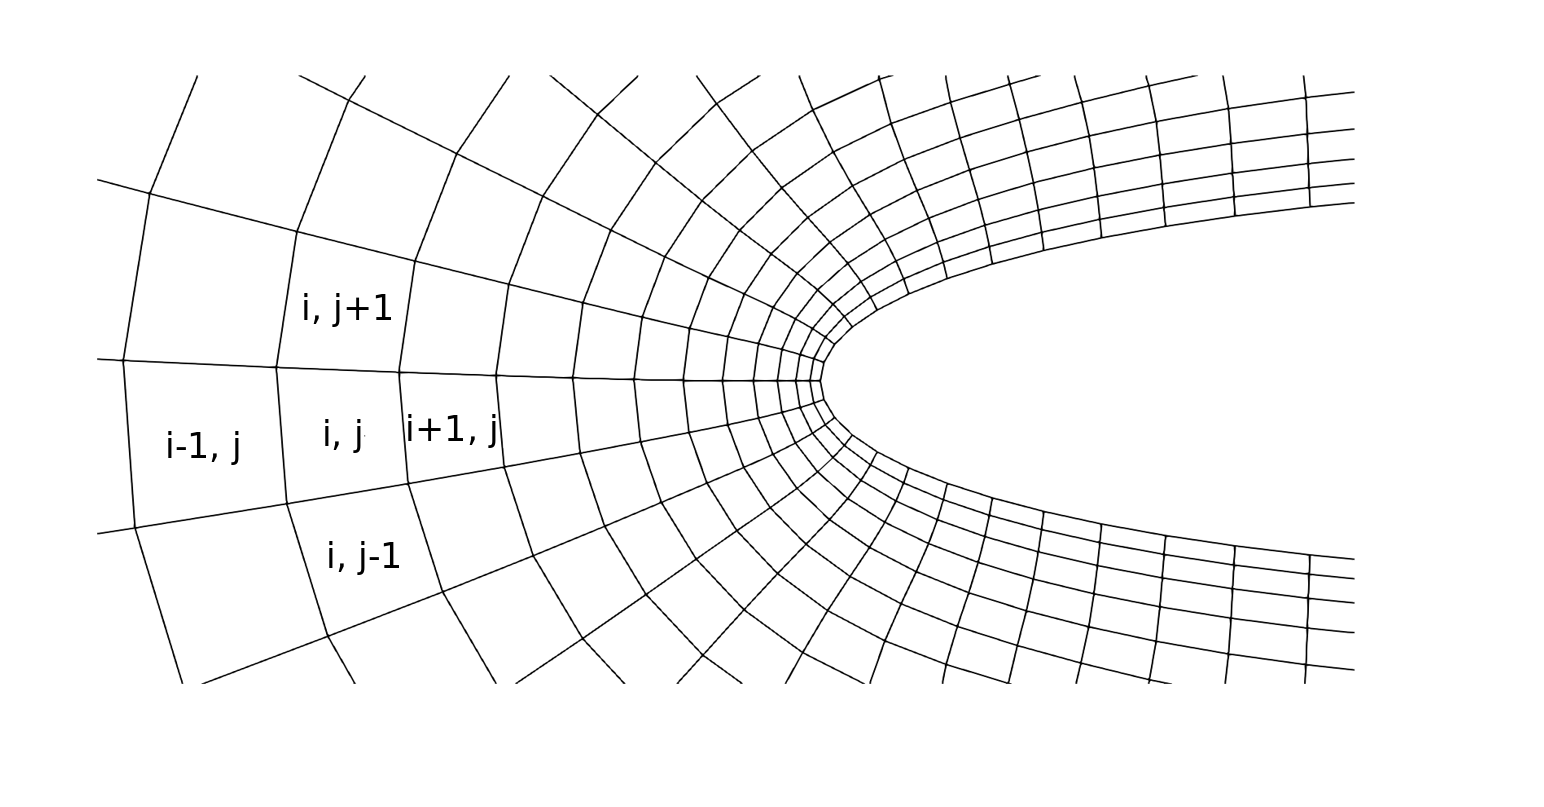
\includegraphics[width=0.8\linewidth]{img/intro/stucturedNaca0012.png}
  \caption{Structured mesh around leading edge of a NACA 0012 airfoil}
  \label{fig-structuredNaca0012}
\end{figure}


Structured meshes were attractive to engineers because of their low memory usage as the topology of the cells is repeated. Also, given simple domains to mesh, these meshes were optimal for minimizing the errors in CFD, resulting in faster simulations \cite{d1991optimal}. Programming CFD solvers with these meshes was easy as cell connectivity occurs in a regular fashion. However, as the scope of CFD simulations grew over time and more complex geometries were becoming commonplace, the task of generating structured meshes around them proved to be a daunting one. 

The disadvantage of using a structured mesh for more complex geometries is the increase in grid non-orthogonality or skewness that can cause unphysical solutions due to the transformation of the governing equations \cite{TU2013219}. The transformed equations that accommodate non-orthogonality act as the link between the structured coordinate system (such as Cartesian coordinates) and the body-fitted coordinate system, but contain additional terms, thereby increasing the cost of numerical calculations and difficulties in programming. Hence, the characteristics of a structured mesh may affect the accuracy and the efficiency of the numerical schemes used by a solver. Additionally, the tedious process of generating such meshes for more complex geometries was hard to justify. Hence, more flexible and automatic methods were devised. These methods produced meshes in a more random manner but with lesser human intervention. Broadly, the meshes produced by such methods were classified as \textit{unstructured meshes}. Figure \ref{fig-unstructured} shows an unstructured mesh. The arrangement of the mesh elements is irregular. Along with the shape of the elements, we need a data structure to store the adjacencies of the mesh.

The cost of finding the flux at a cell boundary, a widely used parameter in Finite Volume Methods (FVM) for fluid flow simulations, for unstructured meshes is high as compared to their structured counterparts. Also, the amount of memory usage is also high as the topology of the mesh is no longer repeated. Still, they are more widely used today because of their capability to handle arbitrary complex geometries, their capability to automate the mesh generation process and their flexibility in refinement based on the geometry and/or the solution gradients. Figure \ref{fig-unstructuredNaca0012} shows an unstructured mesh at the leading edge of a NACA 0012 airfoil. Notice the irregular arrangement of triangles around the airfoil geometry. The connectivity at each vertex of the mesh needs to be stored separately.

\begin{figure}
  \centering
  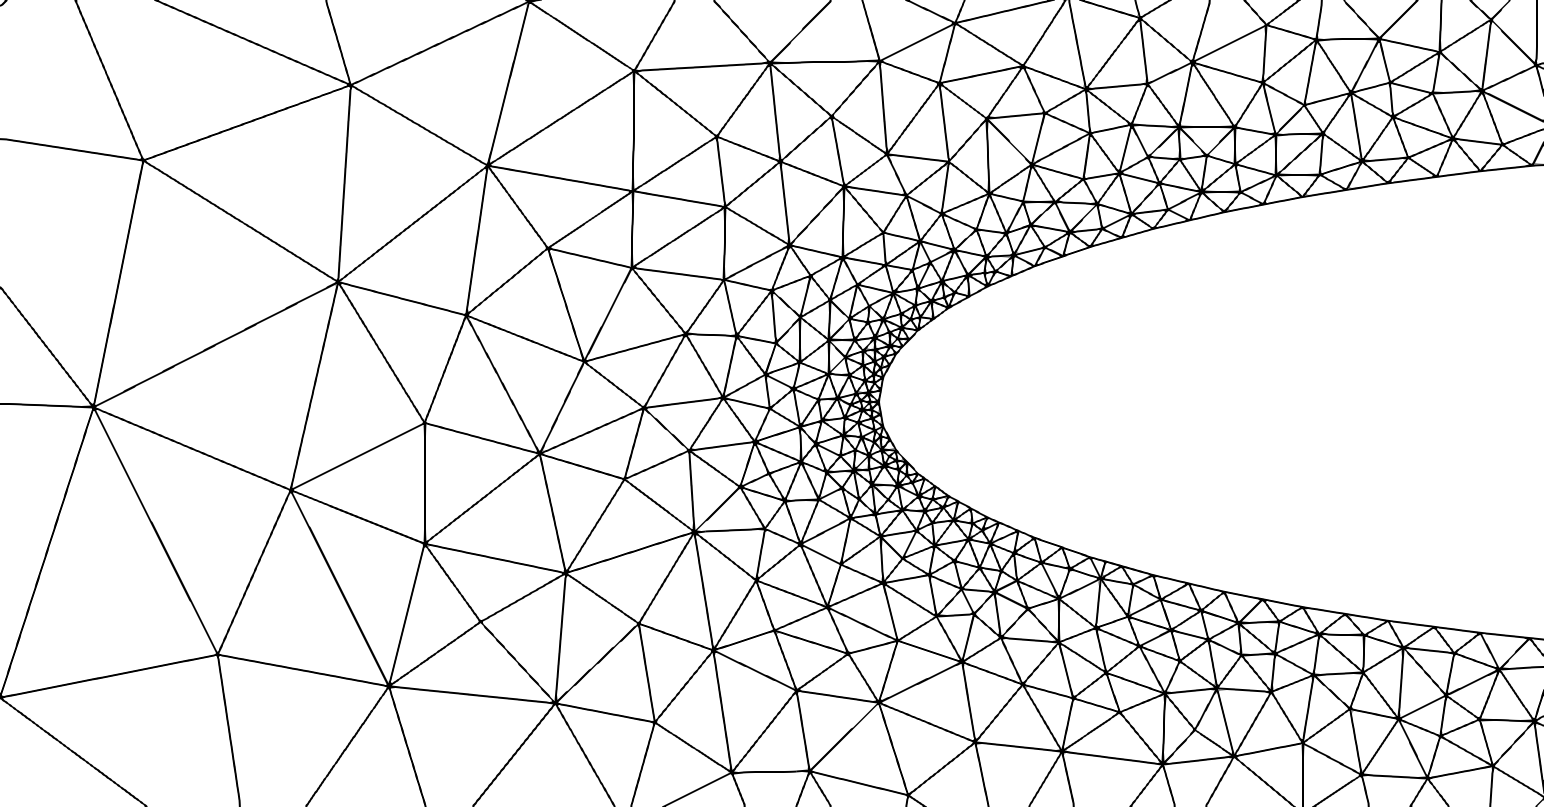
\includegraphics[width=0.8\linewidth]{img/intro/unstructuredNaca0012.png}
  \caption{Unstructured mesh around leading edge of NACA 0012 airfoil}
  \label{fig-unstructuredNaca0012}
\end{figure}

\section{Simplicial and Non-Simplicial Meshes}
\label{sec-simplicial}

Before discussing simplicial and non-simplicial meshes, we need to define certain terms. In geometry, a simplex is a generalization of the notion of a triangle or tetrahedron to arbitrary dimensions. For example, a 0-simplex is a point, a 1-simplex is a line segment, a 2-simplex is a triangle and a 3- simplex is a tetrahedron. See Figure \ref{fig-simplices} for an illustration.

\begin{definition}
A \textbf{k-simplex} is a k-dimensional polytope which is the convex hull of its k+1 vertices
\end{definition}

A simplicial complex is a set composed of points, line segments, triangles, and their n-dimensional counterparts. In other words, a simplicial complex is a set strictly containing simplices only. Figure \ref{fig-simplicialComplex} shows a three-dimensional simplicial complex.

\begin{definition}
A \textbf{simplicial complex} K
is a set of simplices that
satisfies the two following
conditions:
a) Any face of a d-dimensional simplex
 from K is also in K
b) The intersection of any
 two simplices S1 and S2
 is either $\phi$ (null set) or a simplex of dimension $d \leq min(d_1, d_2)$ that is a subset of
 both S1 and S2
\end{definition}

\begin{figure}
	\centering
	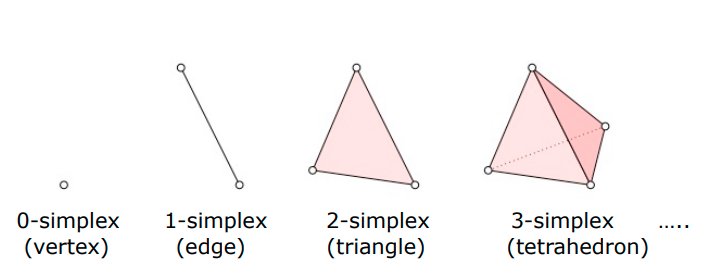
\includegraphics[width=0.95\linewidth]{img/intro/simplices.png}
	\caption{$n$ dimensional simplices.}
	\label{fig-simplices}
\end{figure}

A mesh which contains only simplicial mesh elements is called a simplicial mesh. For example, a mesh which contains only triangular simplices is called a triangulaiton. In other words, a \textbf{triangulation} is the division of a surface or plane polygon into a set of triangles, usually with the restriction that each triangle side is entirely shared by two adjacent triangles. It was proved in 1925 that every surface has a triangulation, but it might require an infinite number of triangles *todo: add citation or omit*. Figure \ref{fig-triangulation} shows a triangulation of a torus.

\begin{definition}
	A \textbf{triangulation} of a topological space X is a simplicial complex K, homeomorphic to X, together with a homeomorphism h: K $\rightarrow$ X.
\end{definition}

A non-simplicial mesh is simply a mesh which is not simplicial. Such a mesh contains mesh elements other than simplices too. For example, in two dimensions, a mesh which contains quadrilateral elements or quads will be called a non-simplicial mesh. In three dimensions, a mesh containing hexahedral elements would fall under the category of non-simplicial meshes.

Simplicial elements have been traditionally used for mesh generation. These elements are simple to work with and provide good flexibility in terms of discretization of a domain. These benefits make simplicial meshes very simple to produce. However, some of the drawbacks of simplicial meshes have led to mesh generation techniques with non-simplicial elements.

Consider a triangulation of a surface. The Euler Formula states that for any convex polyhedron, the number of vertices and faces together is exactly two more than the number of edges. Mathematically,

\begin{equation}
V-E+F=2
\label{eqn-eulerFormula}
\end{equation}

where $V$ is the number of vertices, $E$ is the number of edges and $F$ is the number of faces in the polyhedron. For a triangulation, each edge is shared by two faces. Also, each face has three edges associated with it. Hence, the number of faces is $2/3$ times the number of edges, or $F= (2/3) \times E$. Substituting this in equation \ref{eqn-eulerFormula}, we get

\begin{align}
\begin{split}
		V - E + F  & = 2 \\
		V - E + \frac{2}{3} \: E & = 2 \\
		V - \frac{1}{3} \: E & = 2 \\
		3V & \approx E
		\end{split}
\end{align}

Hence, the number of edges is three times the number of vertices in a triangulation (asymptotically). On the other hand, the number of edges is two times the number of vertices for a closed quadrilateral surface mesh. A similar derivation could be done for three-dimensional simplicial and non-simplicial elements. The number of edges in a tetrahedral mesh is about seven times the number of vertices. On the other hand, in a hexahedral mesh, the number of edges is only about three times the number of vertices (asymptotically). Higher connectivity for simplical meshes leads to higher computational for solving on a given mesh using vertex-based discretization methods. Hence, non-simplicial meshes are substantially more efficient than simplical meshes for a given number of unknowns or grid points.

\begin{figure*}
\begin{minipage}{0.45\linewidth}
	\centering
	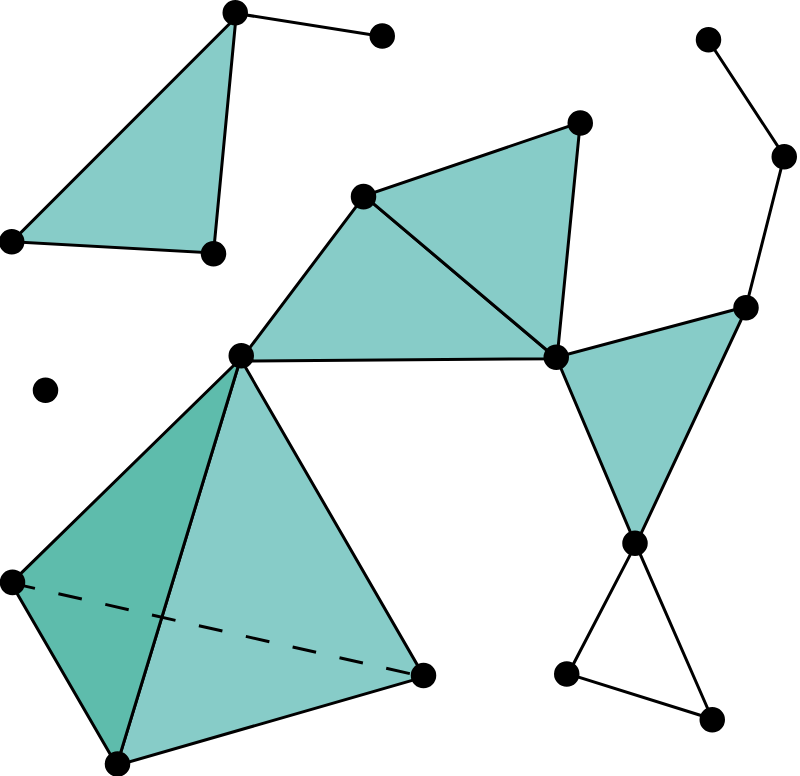
\includegraphics[width=\linewidth]{img/intro/simplicalComplex.png}
	\caption{A three-dimensional simplicial complex.}
	\label{fig-simplicialComplex}
\end{minipage}\hfill
\begin{minipage}{0.45\linewidth}
	\centering
	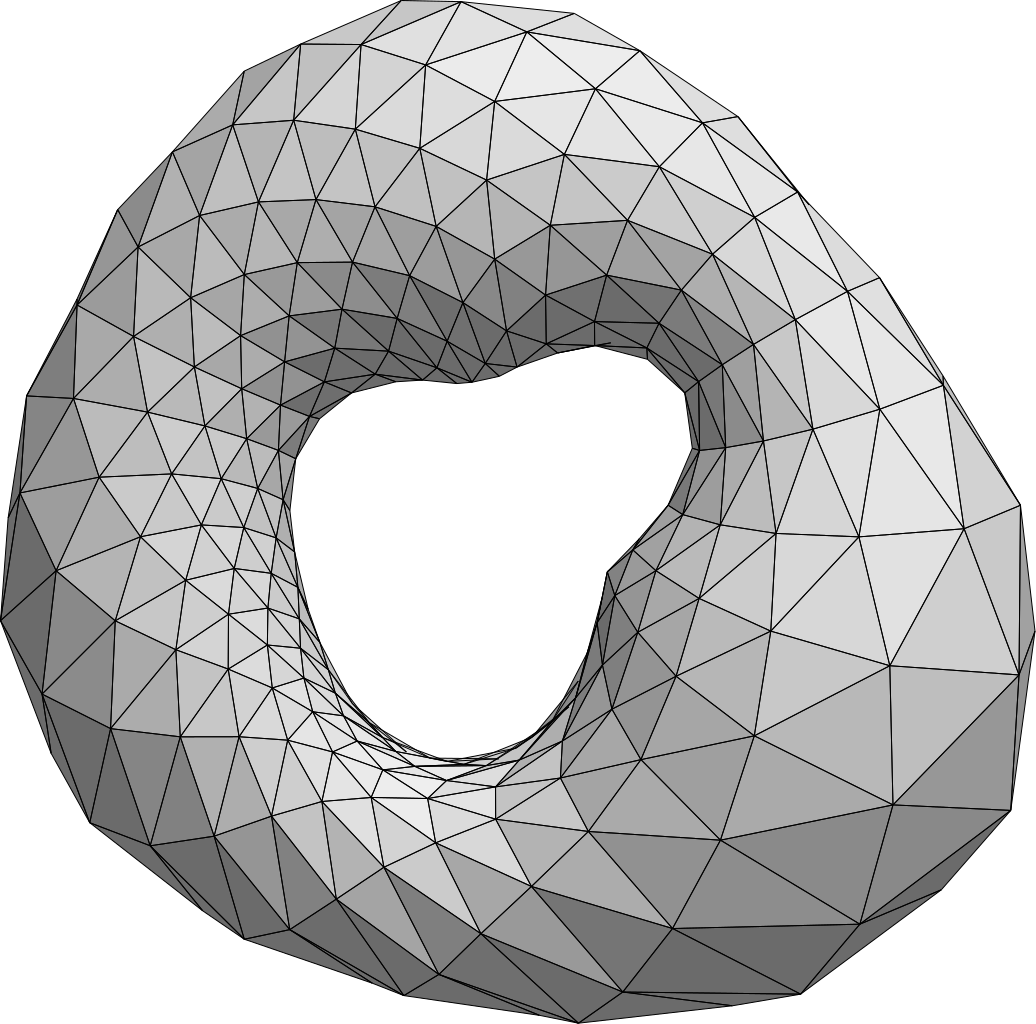
\includegraphics[width=\linewidth]{img/intro/triangulation.png}
	\caption{Triangulation of a torus.}
	\label{fig-triangulation}
\end{minipage}
\end{figure*}

Additionally, regular arrays of nonsimplical elements may also enhance accuracy, owing to a local cancellation of truncation errors that may not occur on groups of nonsimilar simplical elements \cite{mavriplis1997unstructured}. In two-dimensions, quadrilateral elements have been preferred over triangles in highly stretched two-dimensional grids due to their lower connectivity \cite{aftosmis1994accuracy}. These advantages of non-simplical mesh elements have resulted in fully non-simplicial mesh generation techniques \cite{blacker1991paving, zhu1991new}. The scheme introduced by Blacker \etal \cite{blacker1991paving} uses a paving methodology with several mesh element collision checks and special conditions for concave corners to generate an isotropic all-quad two-dimensional mesh for complex geometries. One such mesh is shown in Figure \ref{fig-quadMesh}.

\begin{figure}
	\centering
	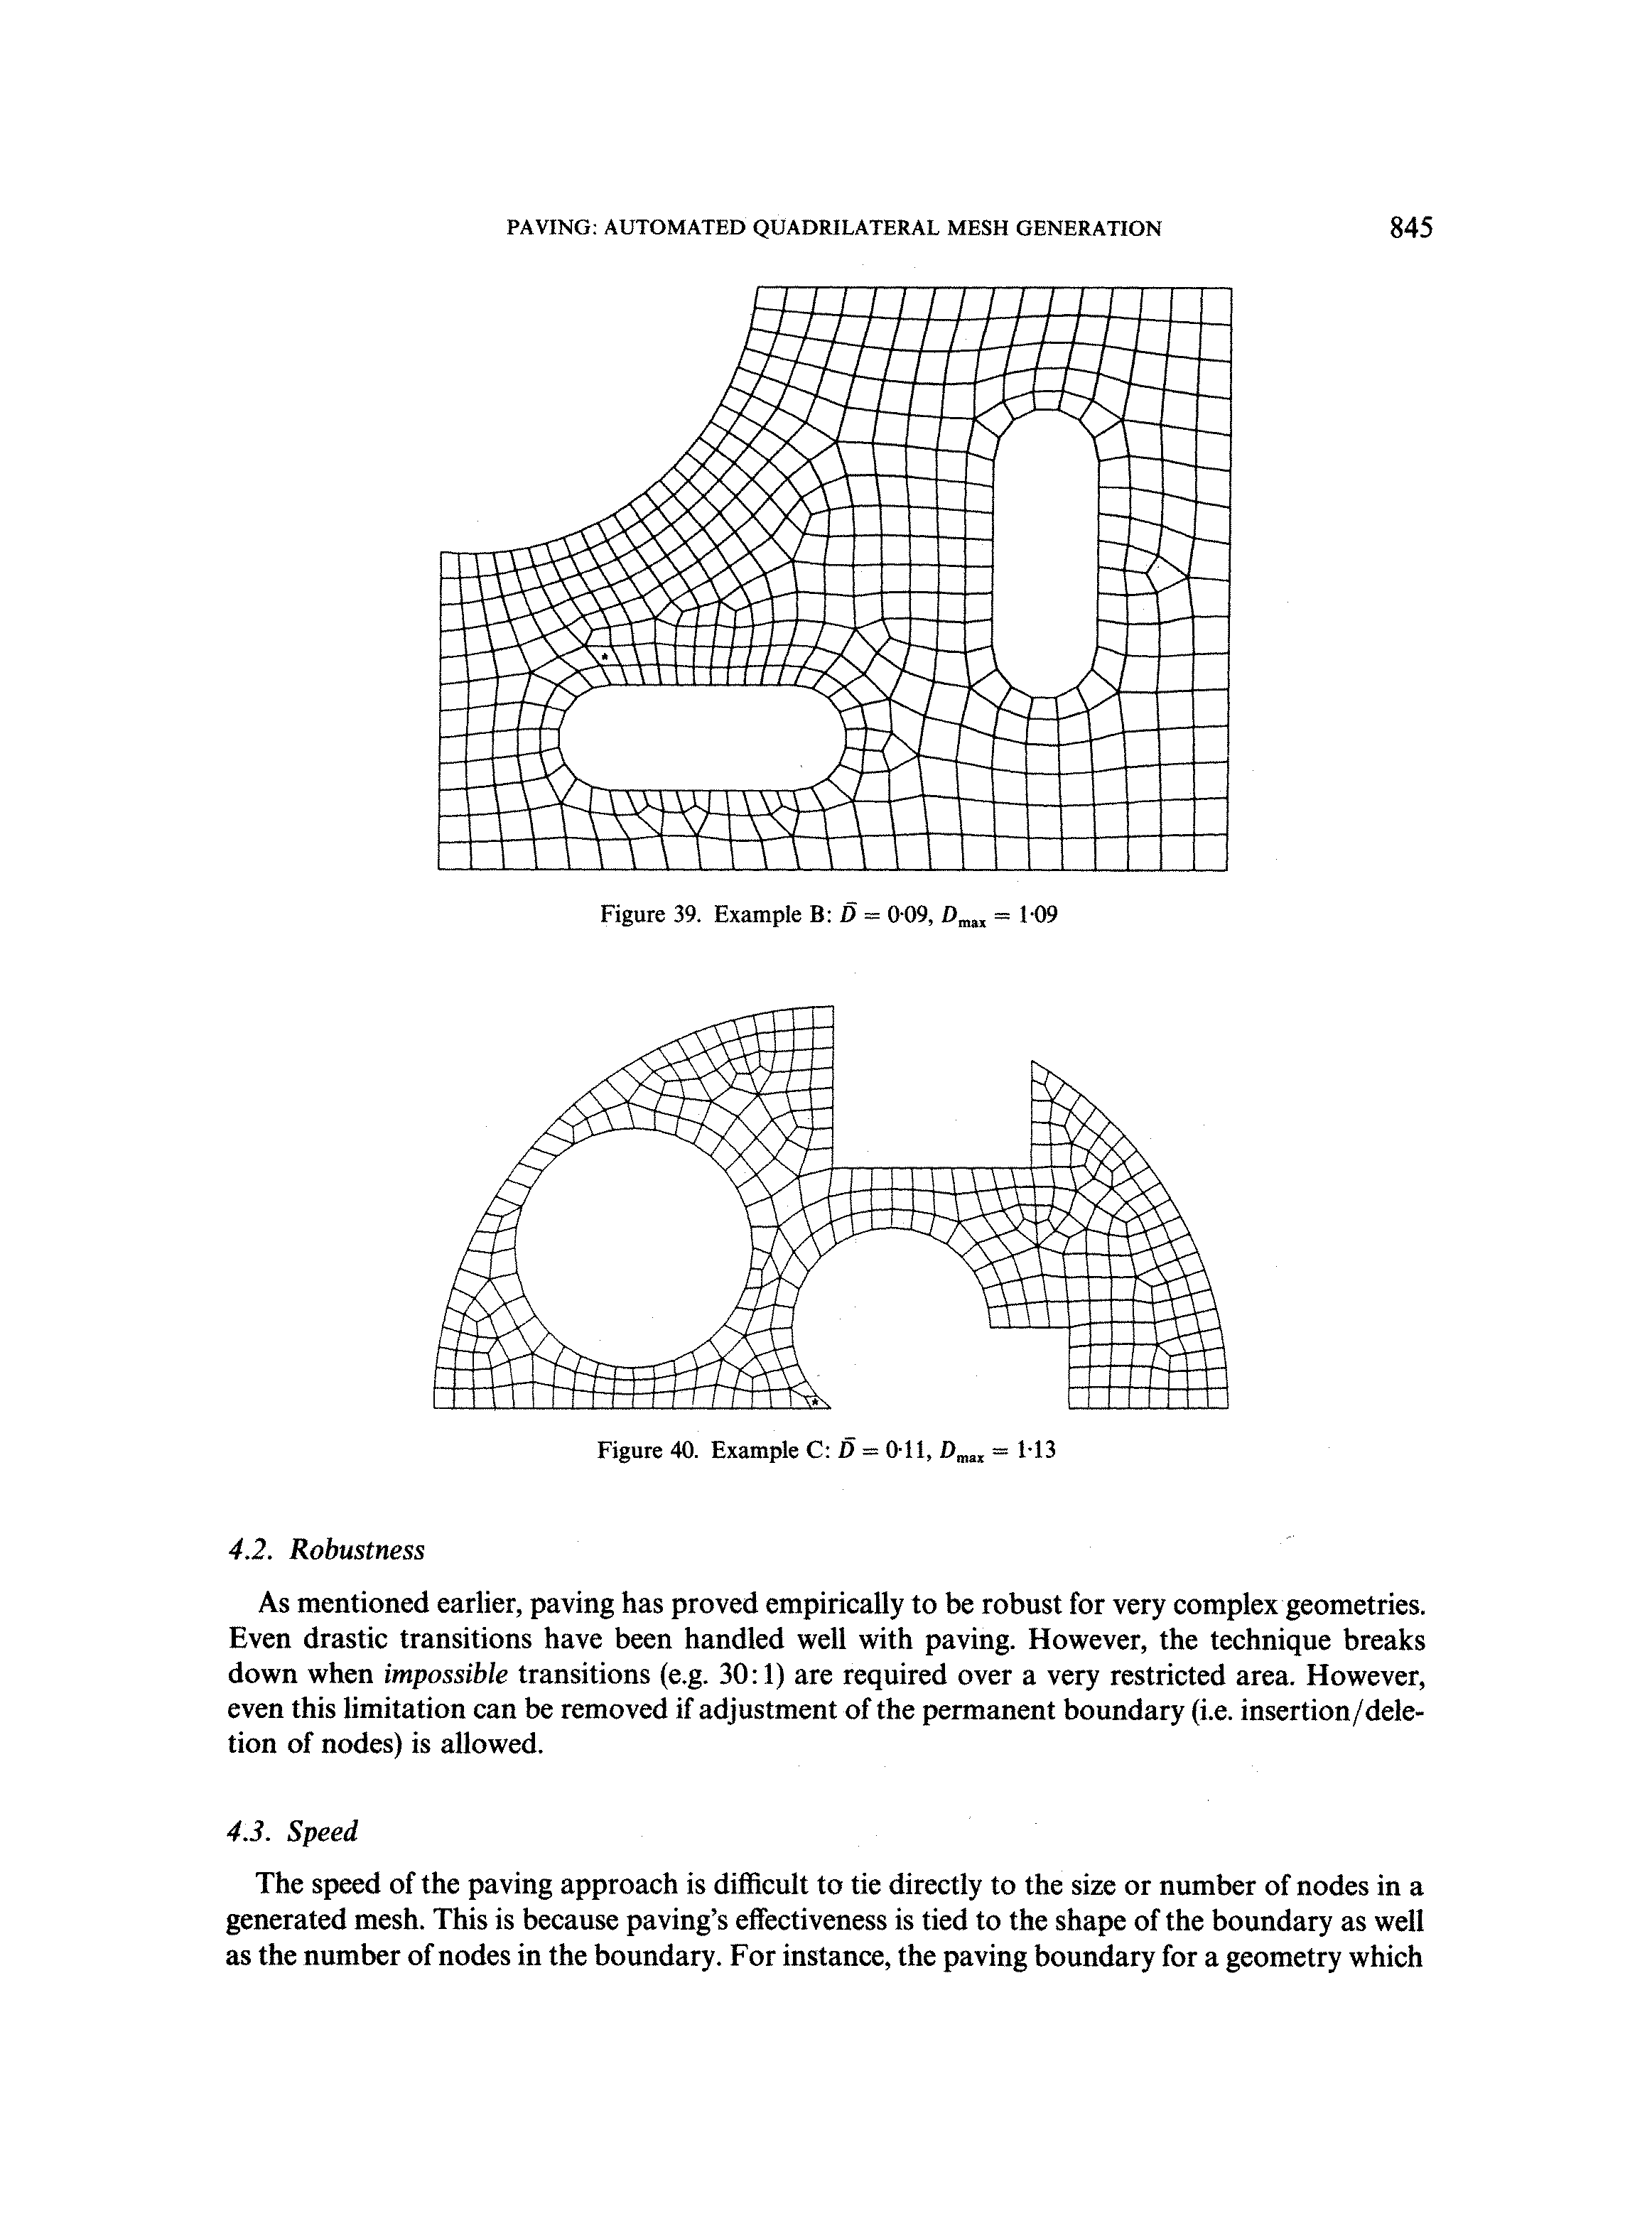
\includegraphics[trim={0 65.5cm 0 14cm },clip,width=\linewidth]{img/intro/lit/quadMesh.png}
	\caption{A non-simplicial quad mesh generated with paving methodology \cite{blacker1991paving}.}
	\label{fig-quadMesh}
\end{figure}

Even though non-simplical mesh elements have been favored for a variety of scenrarios in mesh generation, and especially while generating highly-stretched elements, they have their disadvantages. It is quite difficult to develop an automatic mesh generation strategy which creates non-simplicial meshes conforming to complex surface and 3D geometrical configurations. Manual input is usually required to mesh such geometries. In these situations, simplical mesh elements are quite useful in dealing with the complexity in the geometry. Hence, a hybrid mesh containing both simplical and non-simplical mesh elements is a reasonable choice for mesh generation. We will revisit this in section \ref{sec-motivation} where we reason about choosing a hybrid scheme to mesh the surface.

\section{Boundary Layer Meshes}
\label{sec-boundaryLayerMesh}

With the advent of unstructured mesh generation techniques, a broader selection of geometries could be dealt with. This immensely increased the scope of CFD solvers and pushed the limits of numerical methods in terms of accuracy and speed. However, a different approach was needed for the parts of the mesh in which viscous forces are dominant as compared to the inertial forces. In other words, at the location of the viscous boundary layer, the gradient of physical measures like velocity is several magnitudes higher in one direction as compared to its orthogonal direction. A mesh generation technique which would help in resolving such strong gradients of the velocity in the boundary layer was required. For example, consider a flow over a flat plate as shown in Figure \ref{fig-boundaryLayer}. The velocity of the fluid at the surface of the plate is zero. However, the velocity becomes freestream velocity $u_0$ very near to the surface. The thickness of this layer of fluid, where the velocity of the fluid goes from a value of zero to a value of around 0.99 times the freestream velocity is called the boundary layer thickness $\delta$. It is also called the viscous boundary layer as the viscous effects are dominant in this region of the flow.

\begin{figure}
  \centering	
  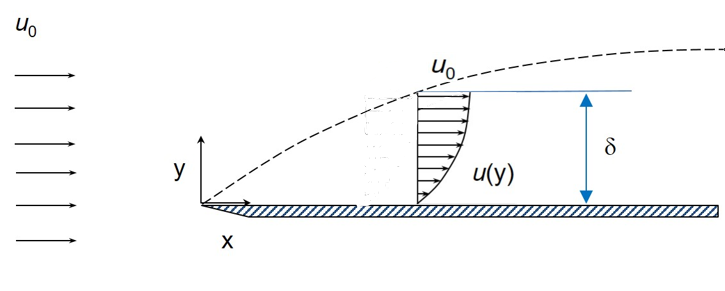
\includegraphics[width=0.8\linewidth]{img/intro/boundaryLayer.png}
  \caption{Fluid flow over a flat plate.}
  \label{fig-boundaryLayer}
\end{figure}

\section{Anisotropic Meshing}

The need to resolve the steep gradients in the boundary layer of the fluid flow gave rise to a type of mesh development strategy called anisotropic meshing. An anisotropic mesh is simply a mesh which has highly stretched elements. In other words, the aspect ratio of the elements for an anisotropic mesh would be very high. Aspect ratio of a mesh element is simply a size measure of the element. For tris and quads, the ratio of the length of the largest edge of the element to the smallest one is usually taken as the aspect ratio of that element. Figure \ref{fig-AR} illustrates some different aspect ratio triangular and quadrilateral elements. 

A highly anisotropic packing of the cell elements provides a large number of Degree Of Freedoms (DOFs) along the direction of steep gradients of physical quantities such as velocity. Traditionally generated isotropic meshes are incapable of resolving such steep gradients \cite{frey2005anisotropic}. *todo: how big is big? that is, what are the typical numbers for aero?* 

\begin{figure}
	\centering
	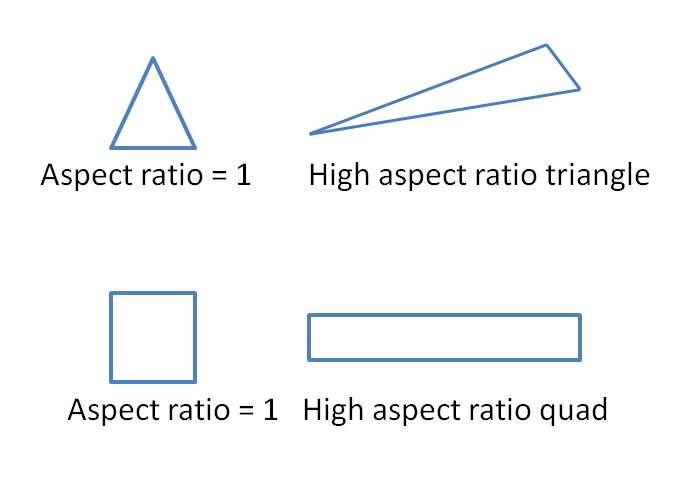
\includegraphics[width=0.6\linewidth]{img/intro/aspectRatio.png}
	\caption{Illustration of different aspect ratio triangular and quadrilateral elements.}
	\label{fig-AR}
\end{figure}

Figure \ref{fig-isotropic} shows an isotropic mesh. The mesh elements have almost equal edge lengths. Here, the mesh elements are triangles and resemble equilateral triangles for most parts of the mesh. Given a point in the mesh, all the directions are the same and there isn't any bias towards a particular direction. For an isotropic physical process, such a mesh will serve the purpose and resolve gradients in all directions given the resolution of the mesh is appropriately chosen. However, if the physical process to be simulated is highly anisotropic, such as the velocity distribution along the boundary layer of the flat plate, as discussed in Section \ref{sec-boundaryLayerMesh}, such a mesh will fail to resolve the steep velocity gradients. It would have to be refined to get the required refinement at the boundary, increasing the total number of DOFs in the mesh by a polynomial factor. Hence, a more reasonable mesh generation strategy is needed.

Figure \ref{fig-anisotropic} shows an anisotropic mesh. The triangular elements of the mesh are highly streched, with one edge being considerably shorter than the other two. The number of DOFs is distributed over the domain in a fashion so as to have the majority of the DOFs along the steep gradients of the physical quantities to be simulated. Hence, cell alignment with the solution to capture anisotropic flow features is possible with such a mesh.

\begin{figure}
	\centering
	\begin{subfigure}{0.5\linewidth}
	  \centering
	  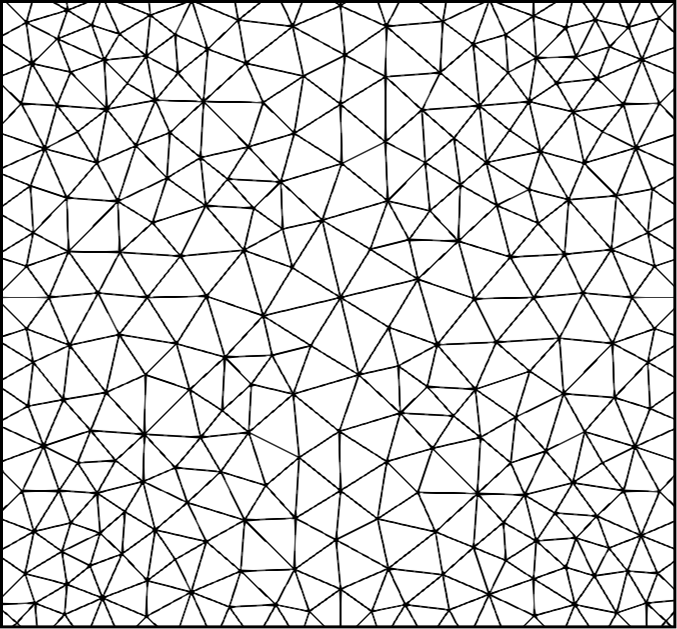
\includegraphics[width=0.9\linewidth]{img/intro/isotropic.png}
	  \caption{Isotropic mesh}
	  \label{fig-isotropic}
	\end{subfigure}%
	\begin{subfigure}{0.5\linewidth}
		\centering
		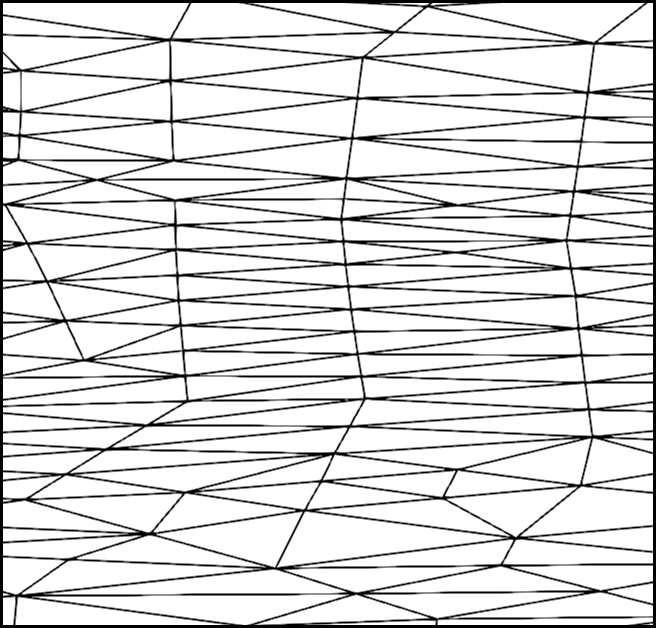
\includegraphics[width=0.88\linewidth]{img/intro/anisotropic.png}
		\caption{Anisotropic Mesh}
		\label{fig-anisotropic}
	\end{subfigure}
	\caption{Isotropic and Anisotropic Mesh Fragments}
	\label{fig-isotropic-anisotropic}
\end{figure}

\subsection{Brief Literature Review - Anisotropic Meshing}

Several techniques have been developed to generate meshes in two dimensions with some sort of anisotropy. Some of these techniques have also been generalized to surfaces. However, isotropically-meshed surfaces with a smooth element-size variation are generally easier to mesh than anisotropically-meshed surfaces with strong size variations \cite{TU2013219}. Many techniques developed in 2D have been generalized to 3D while some new methodologies have been deviced for volume meshing. We go over some of these methods briefly.

\subsubsection{2D and Surfaces}

Most of the initial attempts at generating stretched element meshes in two dimensions used a Delaunay mesh and a locally mapped space to get the required level of anisotropy  \cite{mavriplis1990adaptive}. A mesh generated by such a method is shown in Figure \ref{fig-mavri}. Some techniques used an approach of using a locally structured or semi structured mesh for the regions requiring high anisotropy  \cite{nakahashi1987fdm}.

\begin{figure*}
\centering
\begin{minipage}[b]{.4\textwidth}
	\centering
	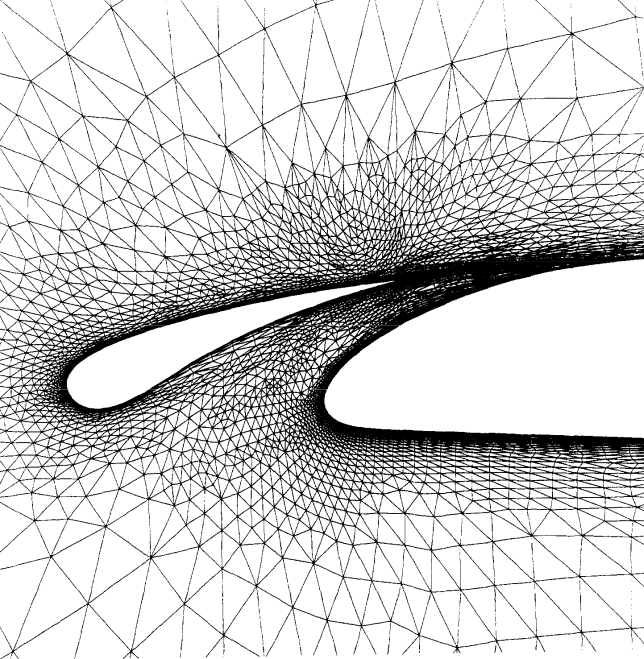
\includegraphics[width=\linewidth]{img/intro/lit/mavri.png}
	\caption{Illustration of adaptively refined mesh for a two-element airfoil configuration near the gap region \cite{mavriplis1990adaptive}.}
	\label{fig-mavri}
\end{minipage}\hfill
\begin{minipage}[b]{.55\textwidth}
	\centering
	\begin{subfigure}{\linewidth}
	\centering
	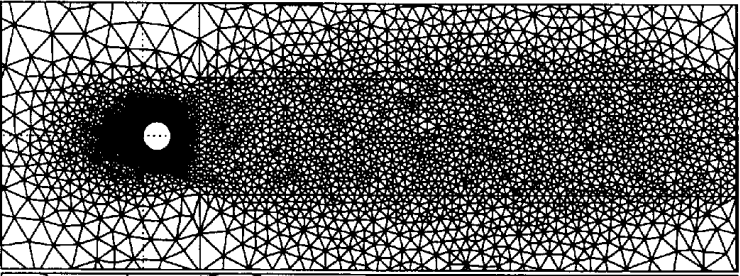
\includegraphics[width=\linewidth]{img/intro/lit/castroInitial.png}
	\caption{}
	\label{fig-castroInitial}
	\end{subfigure}
	\begin{subfigure}{\linewidth}
		\centering
		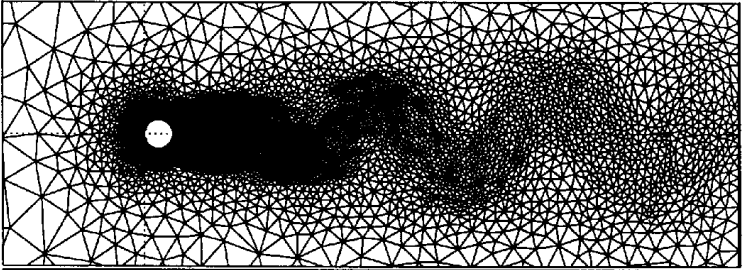
\includegraphics[width=\linewidth]{img/intro/lit/castro.png}
		\caption{}
	\label{fig-castro}
	\end{subfigure}
	\caption{Initial mesh (a) and adaptively generated anisotropic mesh (b) using solution metric evaluation	\cite{castro1997anisotropic}.}
\end{minipage}
\end{figure*}

Many methods for generating anisotropic meshes come under the category of metric adaptation of the mesh. These techniques generally use a Delaunay type initial mesh and refine it anisotropically using a solution metric. Shimada \etal provided an automated method to obtain anisotropic triangulation of a parametric surface. Given a domain geometry and a tensor field that specifies desired anisotropic node-spacing, a proximity-based interacting force field is defined and the force balance configuration is dynamically simulated \cite{shimada1997anisotropic}. Castro \etal applied mesh adaptation technique to generate anisotropic meshes, to compressible viscous flows for a wide range of Reynolds and Mach numbers \cite{castro1997anisotropic}. An illustration of this method can be seen in Figure \ref{fig-castro}. 

Kunert \etal showed an anisotropic mesh generation algorithm that refines the mesh anisotropically by calculating the local error estimate on the initial mesh \cite{kunert2002toward}. This algorithm was presented for both two dimensional and three dimensional meshes. Another mesh adaptation technique by Li \etal tried to align the mesh to a calculated metric tensor from the physics of the problem \cite{li2010anisotropic}. Figure \ref{fig-anisotropicMeshAdaptation} shows one such mesh.

\begin{figure*}
\centering
\begin{minipage}[b]{.44\textwidth}
	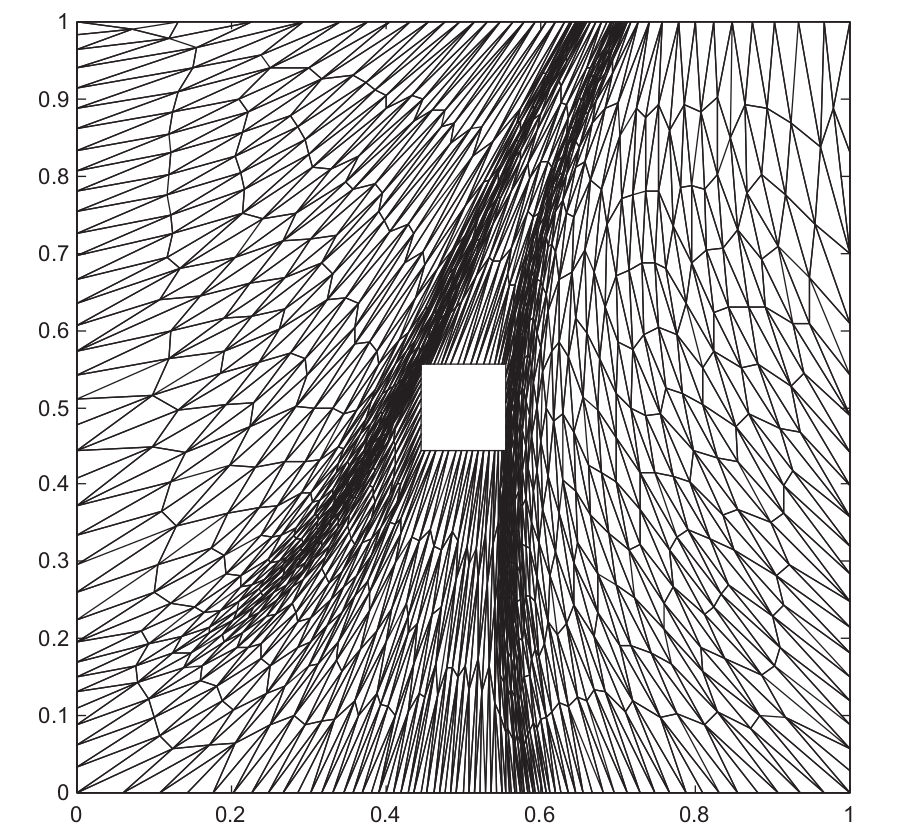
\includegraphics[width=\linewidth]{img/intro/lit/anisotropicMeshAdaptation.png}
	\caption{Anisotropic mesh generated by aligning the mesh elements to a metric calculated from the solution on an isotropic mesh \cite{li2010anisotropic}.}
	\label{fig-anisotropicMeshAdaptation}
\end{minipage}\hfill
\begin{minipage}[b]{.44\textwidth}
	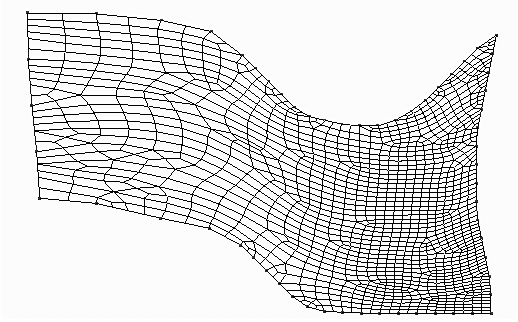
\includegraphics[width=\linewidth]{img/intro/lit/anisotropicQuadMesh.png}
	\caption{Anisotropic quadrilateral mesh generated with an input triangulation and solution contours \cite{viswanath2000quadrilateral}.}
	\label{fig-anisotropicQuadMesh}
\end{minipage}
\end{figure*}

Advancing Layer methods are a practically successful family of anisotropic mesh generation techniques. A method introduced by Pirzadeh produced unstructured triangular/tetrahedral grids with high-aspect-ratio cells using the advancing layer or the grid-marching strategy \cite{pirzadeh1994unstructured}. Another method which used the advancing layer strategy, with several mesh collision checks, was introduced by Lohner \cite{lohner1993matching}. Here, the mesh was produced by inflating the boundary curves in the direction of surface normals. Special care was taken while dealing with the concave corners of the mesh so as to avoid mesh element collisions.



While the majority of anisotropic mesh generation strategies have focused on simplicial mesh elements, there have been some works which generate all quadrilateral (quad) surface meshes. A method by Lee \etal showed an anisotropic quadrilateral mesh generation scheme which generates a background triangular mesh and then uses a cell merging procedure in the parametric space to produce the desired mesh \cite{lee2003new}. A different kind of method was adopted by Viswanath \etal to generate quadrilateral meshes with anisotropy and directional control \cite{viswanath2000quadrilateral}. A 2D geometric domain and desired level of anisotropy - as a metric tensor over the domain, specifying mesh sizing in two independent directions - is taken as an input. Node locations are calculated by closely packing rectangles in accordance with the inputs. An example mesh generated with this strategy is shown in Figure \ref{fig-anisotropicQuadMesh}.

\subsubsection{3D Anisotropic Meshing}
\label{sec-3D}

\begin{figure*}
\begin{minipage}{0.45\linewidth}
	\centering
	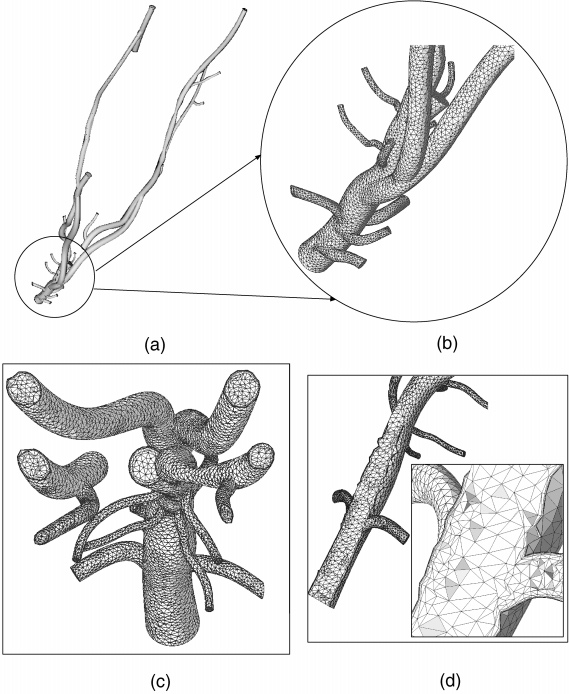
\includegraphics[width=\linewidth]{img/intro/lit/shephard.png}
	\caption{Boundary layer mesh for simulation of ow in blood vessels: (a) geometric model; (b) zoom in of surface mesh in the encircled region; (c);(d) cross-sections showing the boundary layer and isotropic meshes \cite{garimella2000boundary}.}
	\label{fig-shephard}
\end{minipage}\hfill
\begin{minipage}{0.45\linewidth}
	\centering
	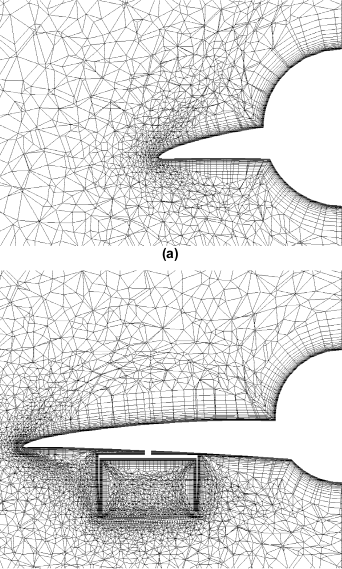
\includegraphics[width=\linewidth]{img/intro/lit/ito.png}
	\caption{Hybrid grid for an aircraft (NAXST-2). Two images show the cross-section of the mesh at two different locations along the chord of the airfoil \cite{ito2002unstructured}.}
	\label{fig-ito}
\end{minipage}
\end{figure*}

Given an initial surface discretization, several 3D mesh generation algorithms have been developed to create anisotropic volume meshes. Many methods which generate two-dimensional anisotropic  meshes can be extended to 3D \cite{lohner1993matching, nakahashi1987fdm,castro1997anisotropic}.

A generalized advancing layer method for generating 3D boundary layer mesh was presented by Garimella \etal \cite{garimella2000boundary}. Model boundaries grow into the domain to fill to generate the mesh in this method. An example mesh can be seen in Figure \ref{fig-shephard}. Another method was introduced by Ito \etal \cite{ito2002unstructured}. Here, a hybrid mesh was generated which comprised of tetrahedra, prisms and pyramids. First, the domain was filled with an isotropic tetrahedral mesh. Subsequently, the boundary walls were shifted inwards and the resulting gap between the tetrahedra and the walls was filled up with prismatic elements. Figure \ref{fig-ito} shows a mesh generated using such a strategy. This mesh generation strategy, of using a highly anisotropic semi-structured mesh near the boundaries of the domain (however, with no gradation over the boundary of the domain), and an isotropic mesh further away from domain boundaries is quite common in 3D meshing. Another example of such a strategy is shown in the work done by Sahni \etal \cite{sahni2008adaptive}. Here, mesh adaptation was applied to a hybrid mesh, with semi-structured stretched elements at the boundary and isotropic elements away from the boundary. Figure \ref{fig-sahni} shows a mesh generated by this method.

\begin{figure}
	\centering
	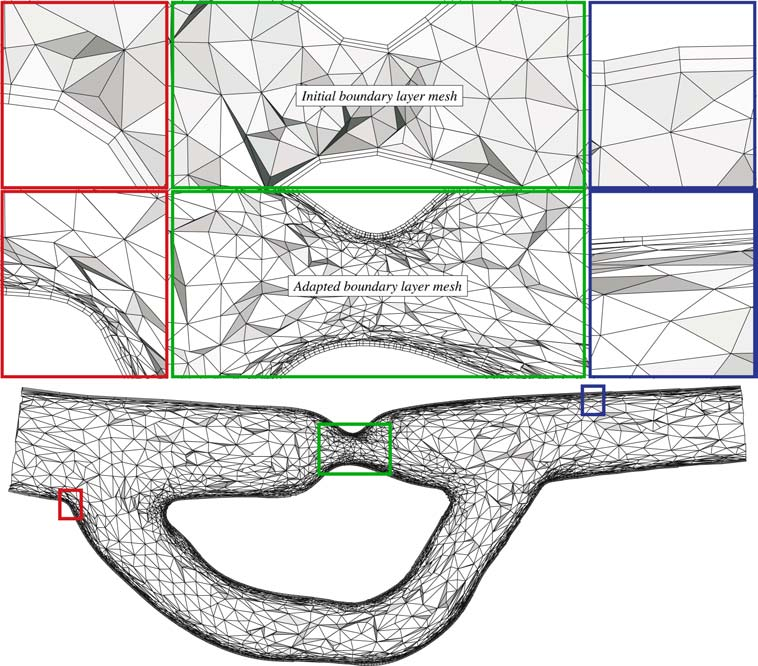
\includegraphics[width=0.8\linewidth]{img/intro/lit/sahni.png}
	\caption{ Collection of mesh faces cut by the vertical center- plane through the adapted boundary layer mesh of a porcine aorta. The windows correspond to magnified views which also show the initial boundary layer mesh \cite{sahni2008adaptive}.}
	\label{fig-sahni}
\end{figure}

The method used by Shimada and Yamada in two dimensions has also been extended to three dimensions to generate anisotropic tetrahedral meshes. Given an arbitrary input anisotropy function, the algorithm generates high quality anisotropic tetrahedral mesh that conforms to the input geometry \cite{yamakawa2000high}. A mesh generated from this method can be seen in Figure \ref{fig-yamakawa}.

\begin{figure}
	\centering
	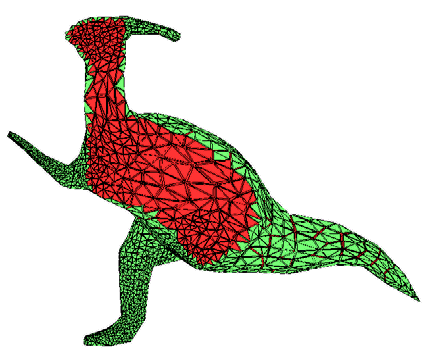
\includegraphics[width=0.5\linewidth]{img/intro/lit/highQualityTetMesh.png}
	\caption{Anisotropic Tetrahedral Mesh generated using ellipsoidal bubble packing methodology  \cite{yamakawa2000high}}
	\label{fig-yamakawa}
\end{figure}

In another work, a metric-orthogonal anisotropic mesh is generated. In addition to aligning the mesh to a metric, mesh elements are also aligned with the eigenvectors \cite{loseille20093d}. The quality of the input metric strongly affects the output mesh.

Another method which generates a hybrid mesh using semi-structured boundary layer mesh and an isotropic outer mesh was given by Ito \etal \cite{ito2007multiple}. Here, special treatment of sharp corners on the surface was done by adding multiple marching directions at the sharp corner. This resulted in generation of a better volume mesh. The research showed that if the corners of the surface mesh, from which the volume mesh is generated, are treated specially and are hence refined more than other regions of the surface, the volume mesh thus generated would be of superior quality. More importantly, such special treatments of sharp corners in the surface mesh helps to create semistructured elements (for viscous boundary layer mesh) around singular points on the surface. A very important problem addressed by this study is one of the pivotal reasons to write this thesis.

Consider Figure \ref{fig-cornerIto} from the work by Ito \etal \cite{ito2007multiple}. An intersection between three surfaces is considered. There are labeled $S_A, S_B$ and $S_C$. The surfaces can represent a wing upper surface, a blunt trailing edge and a fuselage, respectively. As most of the surface meshes are simplical, isotropic and don't treat corners specially, the task to generate a valid viscous boundary layer mesh from them is quite difficult. This difficulty is compounded at complex corners like the one shown in the figure. The paper puts forward a technique to discretize the surface further by adding new nodes and faces to the surface at such corners. In the figure, nodes are added along the direction $BA$. This process helps in creating additional normal directions near the corners of the surface and solves the problem of singularity to a great extent.

\begin{figure}
	\centering
	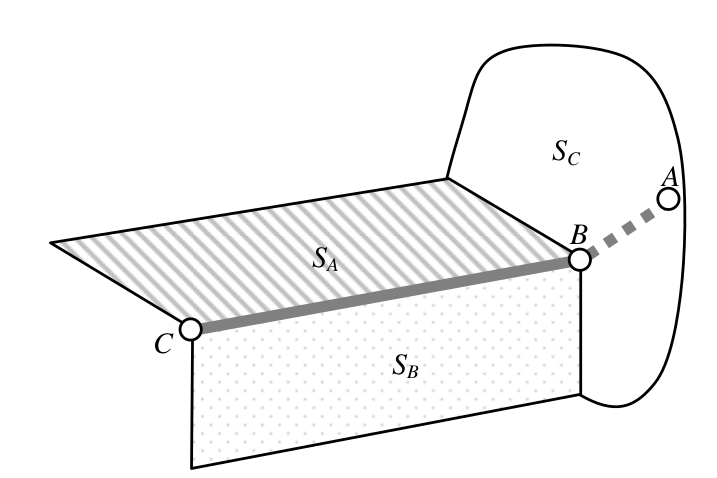
\includegraphics[width=0.8\linewidth]{img/intro/lit/cornerIto.png}
	\caption{Three boundary surfaces $S_A, S_B, $ and $S_C$ \cite{ito2007multiple}}
	\label{fig-cornerIto}
\end{figure}

\section{Motivation}
\label{sec-motivation}

\subsection{Surface Mesh Generation Strategies}

Stretched volume meshes are generated from an initial triangulation of a surface. These surfaces are usually represented by Non-Uniform Rational B-Splines (NURBS) in various Computer Aided Design (CAD) packages. Generation of the surface mesh requires a separate methodology or algorithm as compared to the two-dimensional mesh generation as the mesh elements include a third dimension.

%%Method1

A majority of surface mesh generation methods produce a surface mesh from the parametric mapping of a two-dimensional mesh onto a surface \cite{george1998delaunay, chen1997delaunay}. Usually, a two-dimensional Delaunay mesh is generated over a parametric surface and then mapped onto the curved surface. This method is attractive as it is simple and there are a number of robust Delaunay mesh generation schemes available to generate the initial two-dimensional mesh. However, the mapping from 2D to 3D doesn't always give satisfactory results in terms of mesh element quality. Also, this method doesn't always form well shaped surface elements, especially when the surface derivatives vary over the domain \cite{owen1998survey}. Meshes generated by such methods are generally isotropic and simplical. Hence, in addition to dealing with the badly shaped elements, several other post-processing operations need to be applied to them before generating a boundary layer volume mesh.

%%Method2

A different approach to surface mesh generation is adopted by methods which use the first fundamental form of the surface. In such methods, a metric is derived from the parametric representation of the surface and mesh elements are placed over the surface in an advancing front fashion with respect to this metric. Culli\'ere devised one such method where he used a nodal density function based on the curvature of the surface to discretize it \cite{cuilliere1998adaptive}. An advancing front triangular mesh generation method was presented where 3D parametric surfaces could be meshed with good quality mesh elements. Tristano \etal \cite{tristano1998advancing} presented a method which used a Riemannian surface definition to determine the amount of distortion of the elements in parametric space. An advancing front method is applied to utilize this metric and generate good quality triangular elements over the surface. Figure \ref{fig-joseph} shows a mesh generated with this method. These methods, which use the parametric representation of the surface produce good quality triangular surface meshes. However, they are not well-suited to generate three dimensional anisotropic meshes with highly stretched elements. Additionally, the elements generated by such methods are simplical and hence, have their own drawbacks as discussed in Section \ref{sec-simplicial}.

\begin{figure*}
	\centering
	\begin{minipage}{0.45\linewidth}
		\centering
		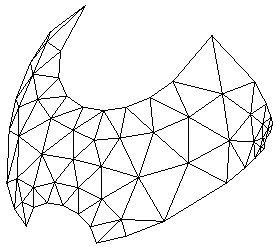
\includegraphics[width=\linewidth]{img/intro/lit/joseph.png}
		\caption{A CAD surface meshed with Reimannian space mesher}
		\label{fig-joseph}
	\end{minipage}
\end{figure*}

%%Method3

Lastly, surface meshes can also be generated by placing the mesh elements directly on the surface of the geometry. Lan and Lu \cite{lan1996finite} provide a method to produce a surface mesh over a given analytical surface. A given element density function is utilized and mesh elements are placed on the analytical surface using the advancing front technique. The elements are optimized considering factors such as surface curvature, element to element turning angle and the given density distribution, to get a high-quality surface mesh. Figure \ref{fig-lu} shows meshes generated with this method. With respect to being an input for a 3D viscous boundary layer mesh, these meshes have similar drawbacks as the ones discussed earlier. Mesh elements generated are triangular rather than quadrilateral or hybrid. Also, there is an additional input required to generate the mesh, which is the density function. Lastly, the boundary curves of the surface are not dealt with specially and the complete surface is isotropically meshed.

\begin{figure}
	\centering
	\begin{subfigure}{0.5\linewidth}
		\centering
		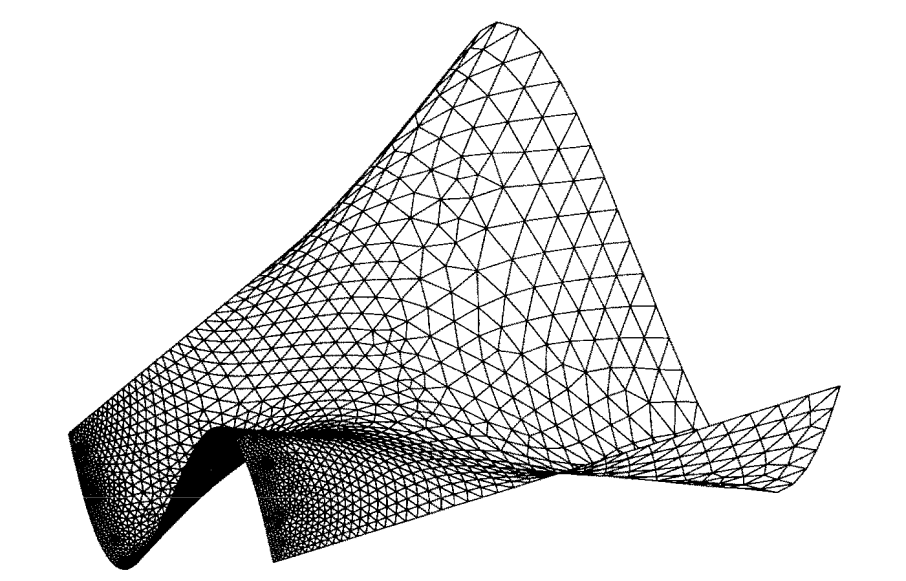
\includegraphics[width=\linewidth]{img/intro/lit/lu1.png}
		\caption{A ruled surface.}
		\label{fig-lu1}
	\end{subfigure}
	\begin{subfigure}{0.5\linewidth}
		\centering
		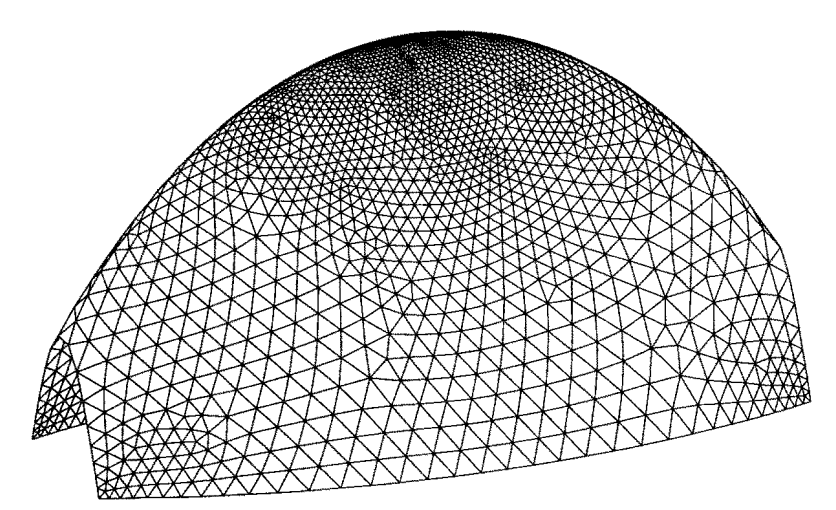
\includegraphics[width=\linewidth]{img/intro/lit/lu2.png}
		\caption{A free form surface.}
		\label{fig-lu2}
	\end{subfigure}
	\caption{Meshes generated directly over the surface by utilizing the analytical surface representation and element density distribution \cite{lan1996finite}.}
	\label{fig-lu}
\end{figure}

%%Consolidating

\subsection{Consolidating The Discussion}
\label{consolidate-motivation}

%% 1. Hybrid
\subsubsection{Hybrid Meshing}
Consolidating our discussion on surface meshes, we find that most of the 3D surface meshes generated are triangular. In other words, these meshes are simplical. We discussed the pitfalls of using simplical mesh elements at the regions of anisotropy or at surface boundaries in Section \ref{sec-simplicial}. To recapitulate, higher vertex connectivity for simplicial meshes makes them inefficient when using a vertex-based discretization method. On the other hand, quad meshes in two dimensions and hex meshes in 3D are substantially more efficient than their simplicial counterparts for the same number of Degrees of Freedom. Non-simplicial quadrilateral elements have been preferred over triangles in highly stretched two-dimensional grids due to their lower connectivity \cite{aftosmis1994accuracy}. In addition to that, non-simplicial elements arranged in repeating arrays may enhance solution accuracy by local cancellation of truncation errors while their simplicial counterparts may fail to do so \cite{mavriplis1997unstructured}.

Even though non-simplicial elements are more efficient for flow solution, conforming such elements to complex geoemtry remains a daunting task. Generally, manual input is required to generate all-quad surface meshes or all-hex volume meshes in the regions of geometric complexities. Hence, usage of simplicial mesh elements in these regions is a reasonable alternative. Hence, a surface mesh generation scheme is required, that generates a quad-dominant mesh with a very limited number of triangular elements. Regular arrays of highly-stretched quadrilateral elements should form the anisotropic boundary layer mesh. On the other hand, triangular elements could be used whenever one wants to conform to the geometry and increase the quality of the mesh elements generated.

%% 2. 3D
\subsubsection{Good Input For Anisotropic 3D Meshing}
Following the discussion from \ref{sec-3D}, it is particularly difficult to generate  hybrid 3D meshes from an isotropic surface discretization. At the minimum, several validation checks needs to be performed at the singularity points of the surface so as to generate a valid viscous 3D mesh. In addition to that, the anisotropy of the 3D mesh becomes extremely difficult to control at the complex corners of the surface if they are not handled specially. One solution discussed earlier was to add additional marching directions and nodes at the complex corners on the surface of the mesh so as to add additional normal directions near the complex corners. However, the root cause of the problem is the isotropic surface discretization which is completely unaware of its usage into a anisotropic 3D volume mesh generator. Hence, a better alternative is desirable which automates the process of special treatment of surface cusps.

%% 2. Automatic and Flexible
\subsubsection{Automatic + Flexibility}

Surface mesh generation methodologies either have several assumptions on the type of surfaces they can support or need a considerable amount of human intervention to complete. Especially for the cases where complex corners exist on the surface, a good surface mesh would need special arrangement of nodes and marching directions on the surface so as to produce a high-quality anisotropic volume mesh. Block structured meshes could be produced on a surface by manually discretizing the domain into several subdomains and meshing them using structured mesh generation technique independently. But again, the mesh generation process would be very tedious and would take a considerable amount of manpower. Hence, an automatic mesh generation technique which has a good level of anisotropy at surface boundary curves is desirable to serve as a good input to 3D mesh generation. Lastly, the mesh generation process should be flexible in terms of the surface representation it can accept as an input. Many methods discussed earlier use the parametric form of the surface to generate the mesh. Additionally, some methods also require an element density distribution to be specified for the entire domain of the surface which needs to be meshed. These constraints again make it cumbersome to generate good quality surface meshes (for anisotropic volume meshes) for a wide variety of surface topologies. Hence, a method of surface mesh generation which accepts a more widely used surface representation is highly desirable.

\subsection{Entire Domain Advancing Layer - Surface Mesh (EDAM-S) Generation}

We present a surface mesh generation algorithm that serves to address the aforementioned issues and has the desired qualities. The algorithm generates a surface mesh which has anisotropic characteristics normal to the boundary curves of the surface. The mesh elements are highly stretched at these boundary curves of the surface and have a required level of directional anisotropy normal to the boundary curves. For the examples in this thesis, the boundary curves of the surface are chosen to be the curves where the surface normal direction jumps abruptly. Practically, the algorithm is independent of the selection of the boundary curves and can work for any selected set of boundary curves for a given surface. However, for the sake of automation and simplicity, the boundary curves are chosen to be the sharp features on the surface topology.

The surface discretization produced by the algorithm given in the thesis consists of a hybrid grid. Most of the elements (usually greater than 95\%) are quadrilateral mesh elements. A regular pattern of quad elements is repeated from the boundary curves of the surface towards its interior. This pattern helps retain the boundary curve topology towards the interior regions of the mesh. In addition to that, an appropriate discretization of the boundary curves of the surface can provide several additional normal directions to the surface near the boundary curves. This may be vital in solving the problem of complex corners or singularity points on the surface while generating a 3D viscous volume mesh.

While most of the elements in the mesh are non-simplicial, some triangular mesh elements are also utilized to discretize the surface. These elements are quite useful when dealing with complex surface topologies such as concave corners. Additionally, triangular mesh elements help to control the growth of the aspect ratio of the mesh elements as the mesh proceeds from the boundary towards surface interior. Overall, the surface mesh hence generated utilizes the advantages of both simplicial and non-simplicial elements. As the surface mesh produced is quad-dominant, it can be used to produce a hex-dominant volume mesh (for anisotropic boundary layer meshes or otherwise).

To keep the mesh development algorithm flexible and simplify the mesh generation pipeline, the input to the mesh generation scheme is only the initial surface triangulation as a stereolithography (STL) file. STL files are the standard in 3D printing and CAD packages. These files contain the information regarding all the triangles in the mesh. Each triangle contains its normal and coordinates of its vertices. Hence, these files are easy to generate and use. Additionally, it is easy to generate a surface triangulation from a parametric or analytic representation of the surface. Innumerable surface triangulation packages are available to generate isotropic and triangular surface discretization with the given amount of refinement. Hence, taking a surface triangulation as an STL file is a reasonable choice for generating the desired surface meshes.

The surface mesh generation technique described in the thesis is based on a closed advancing front method. The surface triangulation imported to the mesh generator is taken as the initial mesh and mesh elements are placed over it to generate the desired surface mesh. The method needs minimal user input and automatically generates an advancing layer mesh from a given input surface triangulation. The only primary user input in addition to the surface triangulation are the initial extrusion length $x$ of the surface mesh and the growth ratio $g$. The initial extrusion length, $x$, defines the thickness of the first layer of the surface mesh. If a user defined value is not provided, the mesh generation algorithm makes a reasonable assumption and proceeds to mesh the domain. 

Sequentially, the input surface is first segmented into several sub-surfaces so that each of them can be meshed independently. Boundary curves of the surfaces are identified and the points on the boundary curves iteratively march towards the interior of the surface. Initial extrusion length and growth ratio can be varied so as to give the required level of anisotropy at each point of the mesh or for a given boundary curve. A valid surface mesh is produced after each layer is marched from the boundary curves. This gives the user freedom to advance until a given level of anisotropy is attained or until the advancing front routine terminates itself. 

Several quality checks and improvements are made during the mesh generation process. These include controlling the element to element turning ratio, limiting the deviation of the mesh elements from the underlying surface (or rather, sub-surface), swapping of edges so as to increase element quality, edge collapse to control aspect ratio and improve element quality, smoothing, and special handling of corners. All these subroutines play a vital role in the overall mesh generation process.

However important may the advancing layer surface mesh generation process described here be, its creation poses challenges for geometries that are highly complicated and/or highly curved. In addition to that, tackling sharp concave corners on a surface mesh is a challenge in itself. These challenges raise robustness issues for most of the mesh generation procedures. Our advancing front routine includes several validity checks to avoid these issues. However, a completely robust algorithm which could generate an anisotropic surface mesh for all such complicated topologies is still a work in progress.

\section{Outline}

************************************************************** \\
Outline will be updated as I complete various chapters of the paper.
Also, is it fine to place the outline of the thesis at this location? For me, this was fine as I could not place it before without breaking the flow of the chapter. \\
**************************************************************

